
\chapter{Bedienoberfläche}

	\paragraph{/B10/ Alle offenen Spielräume müssen angezeigt werden.}\hspace{1mm}\\
	\paragraph{/B20/ Die Spielrauminformationen müssen angezeigt werden.}\hspace{1mm}\\
	\paragraph{/B30/ Gesendete Nachrichten werden im ausgewählten Chat bei allen Teilnehmern angezeigt.}\hspace{1mm}\\
	\paragraph{/B40/ Highscoretabelle soll auf Anfrage angezeigt werden.}\hspace{1mm}\\
	\paragraph{/B50/ In einem Spielraum werden die eigenen Handkarten mit ihren jeweiligen Werten angezeigt.}\hspace{1mm}\\
	\paragraph{/B60/ In einem Spielraum sind Handkarten der Gegner nur mit dem Kartenrücken darzustellen.}\hspace{1mm}\\
	\paragraph{/B70/ In einem Spielraum werden Nachrichten der Spielergruppe im dazugehörigen Chatfenster angezeigt.}\hspace{1mm}\\
	\paragraph{/B80/ In einem Spielraum werden Karten, die bereits auf einem Stichstapel liegen verdeckt angezeigt}\hspace{1mm}\\
	\paragraph{/B90/ In einem Spielraum sind Informationen zu den Spielern und dem Spiel anzuzeigen}\hspace{1mm}\\
		\begin{itemize}
			\item Benutzername
		\end{itemize}
		\begin{itemize}
			\item Punktestand
		\end{itemize}
		\begin{itemize}
			\item Spielmodus
		\end{itemize}
	\paragraph{/B90/ Es wird angezeigt, welcher Spieler an der Reihe ist.}\hspace{1mm}\\
	\paragraph{/B100/ In einem Spielraum werden Karten, die sich in einem Stich befinden, sichtbar für alle Spieler angezeigt.}\hspace{1mm}\\
	\paragraph{/B110/ In einem Spielraum werden nach jeder Spielpartie Spielstatistiken angezeigt}\hspace{1mm}\\
	
\begin{center}
	\begin{figure}[h]
		\hspace*{-1.5cm}
		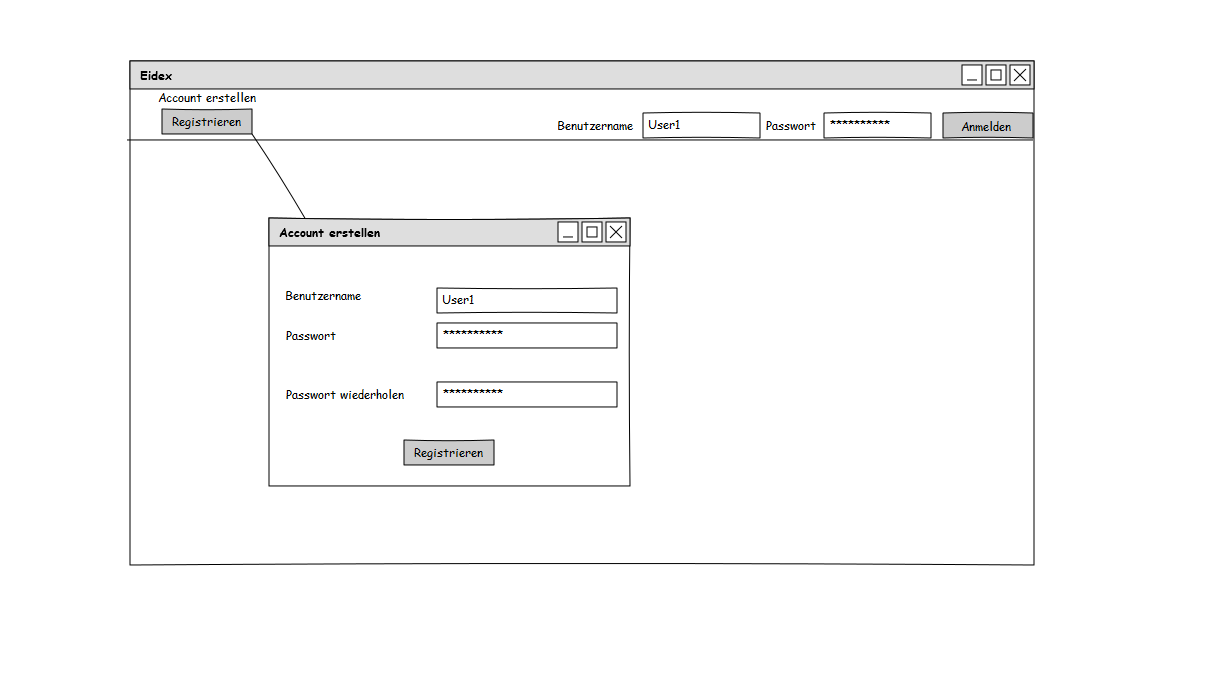
\includegraphics[width=170mm, height =140mm]{PencilProjectData/logging1}
		\caption{GUI Logging}
	\end{figure}
	
	
	
	\begin{figure}[h]
		\hspace*{-1.75cm}
		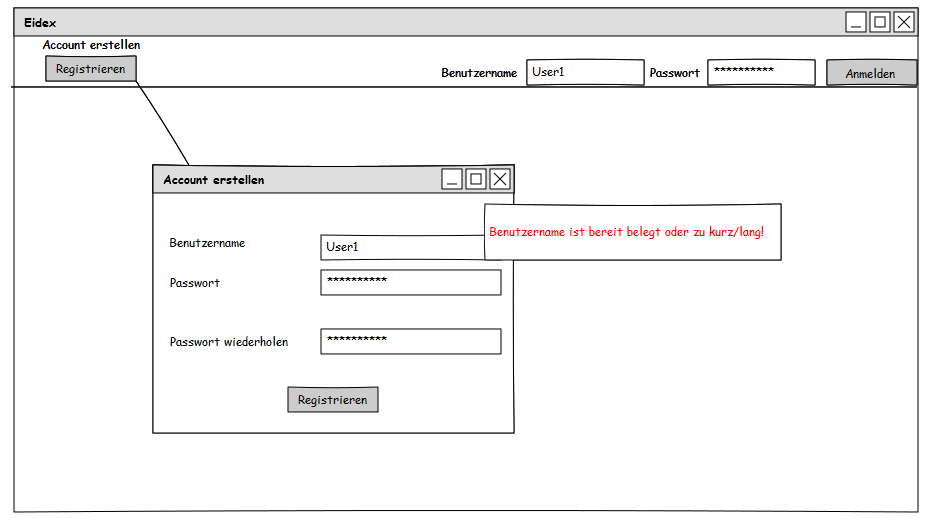
\includegraphics[width=170mm, height =140mm]{PencilProjectData/logging2}
		\caption{GUI Logging}
	\end{figure}
	
	
	\begin{figure}
		\hspace*{-1.9cm}
		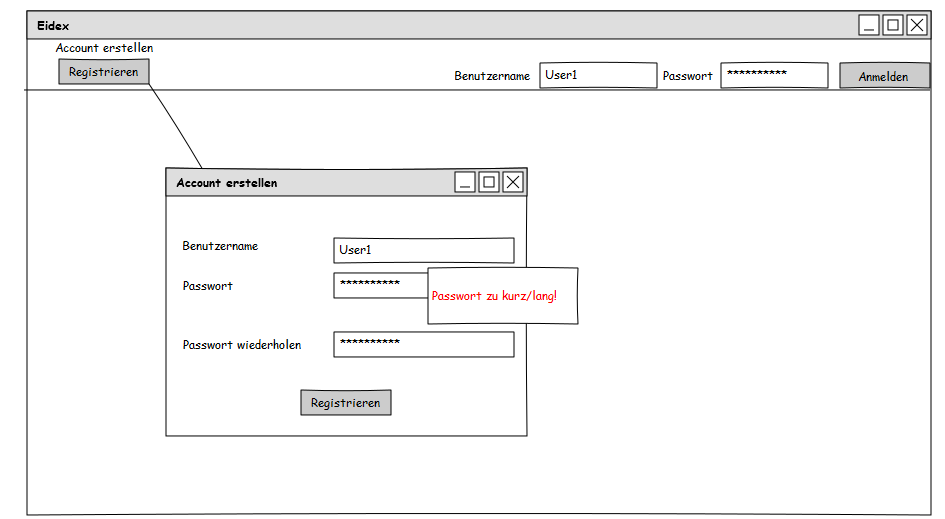
\includegraphics[width=170mm, height =140mm]{PencilProjectData/logging3}
		\caption{GUI Logging}
	\end{figure}
	
	\begin{figure}
		\hspace*{-2cm}
		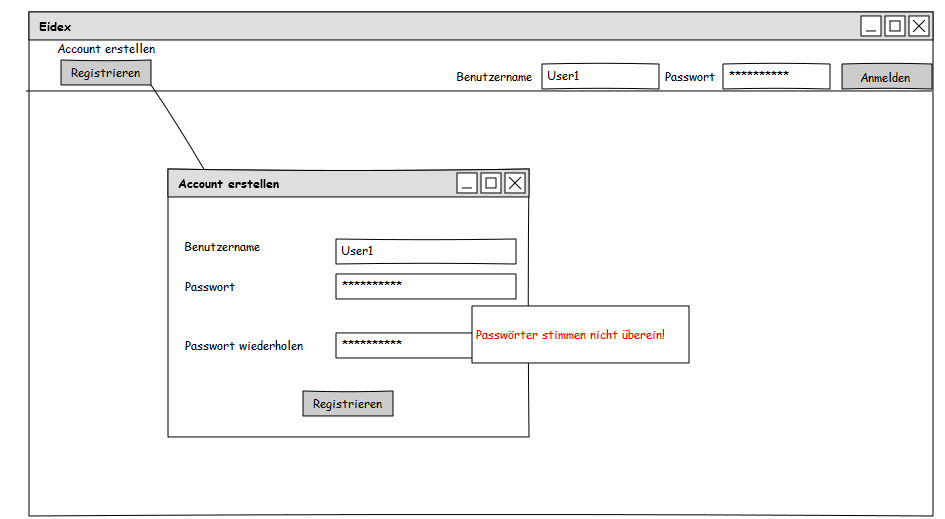
\includegraphics[width=170mm, height =140mm]{PencilProjectData/logging4}
		\caption{GUI Logging}
	\end{figure}
	
	\begin{figure}
		\hspace*{-1.75cm}
		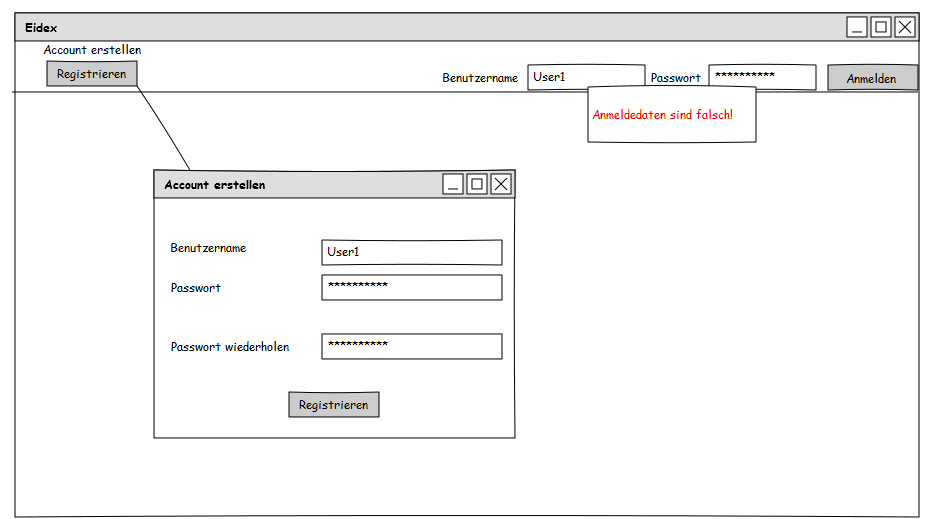
\includegraphics[width=170mm, height =140mm]{PencilProjectData/logging5}
		\caption{GUI Logging}
	\end{figure}
	
	\begin{figure}
		\hspace*{-1.5cm}
		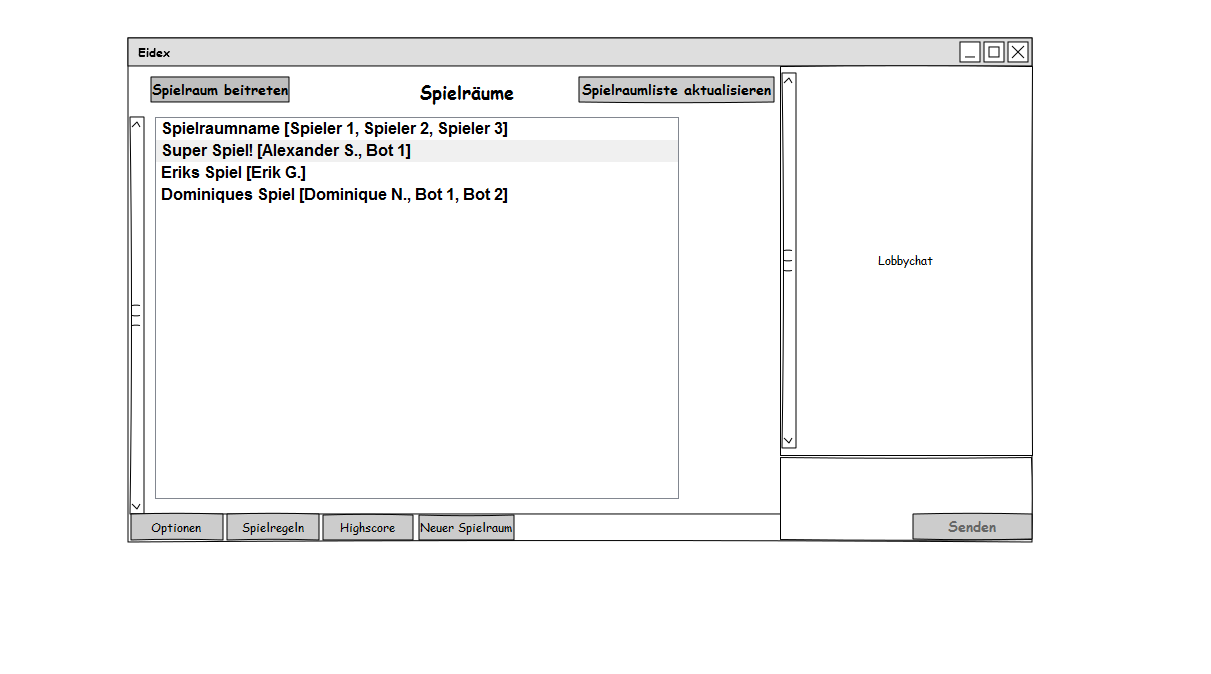
\includegraphics[width=170mm, height =140mm]{PencilProjectData/lobby1}
		\caption{GUI Lobby}
	\end{figure}
	
	\begin{figure}
		\hspace*{-2cm}
		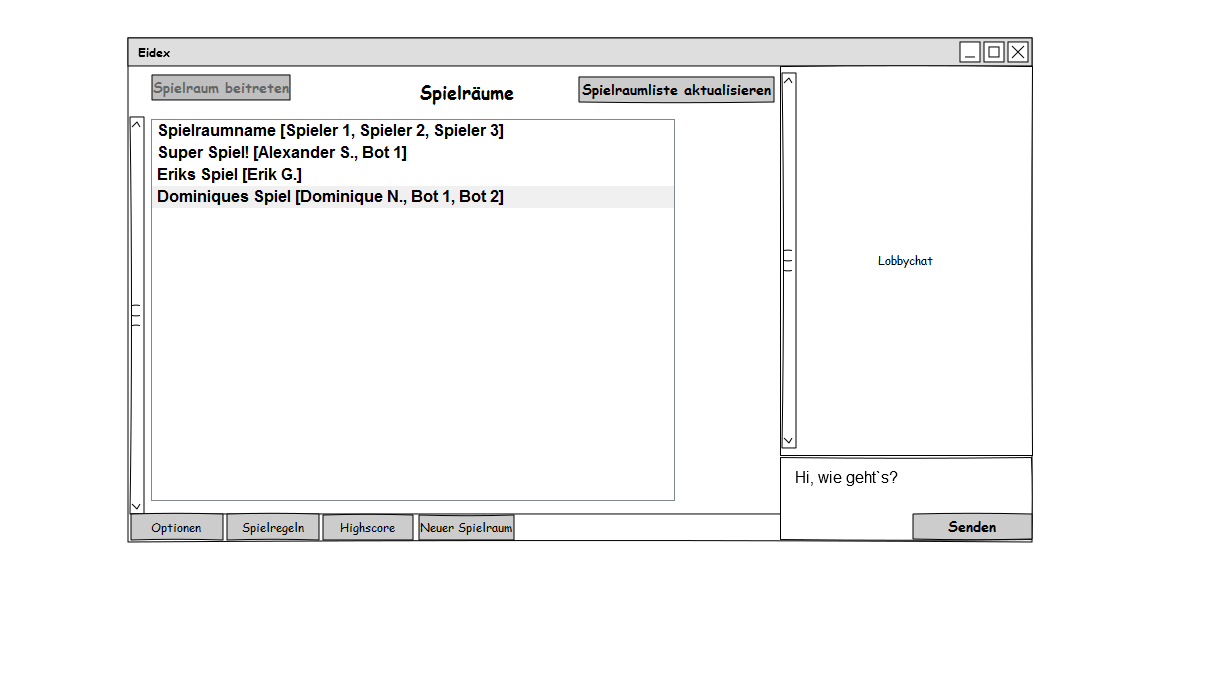
\includegraphics[width=170mm, height =140mm]{PencilProjectData/lobby2}
		\caption{GUI Lobby}
	\end{figure}
	
	\begin{figure}
		\hspace*{-1cm}
		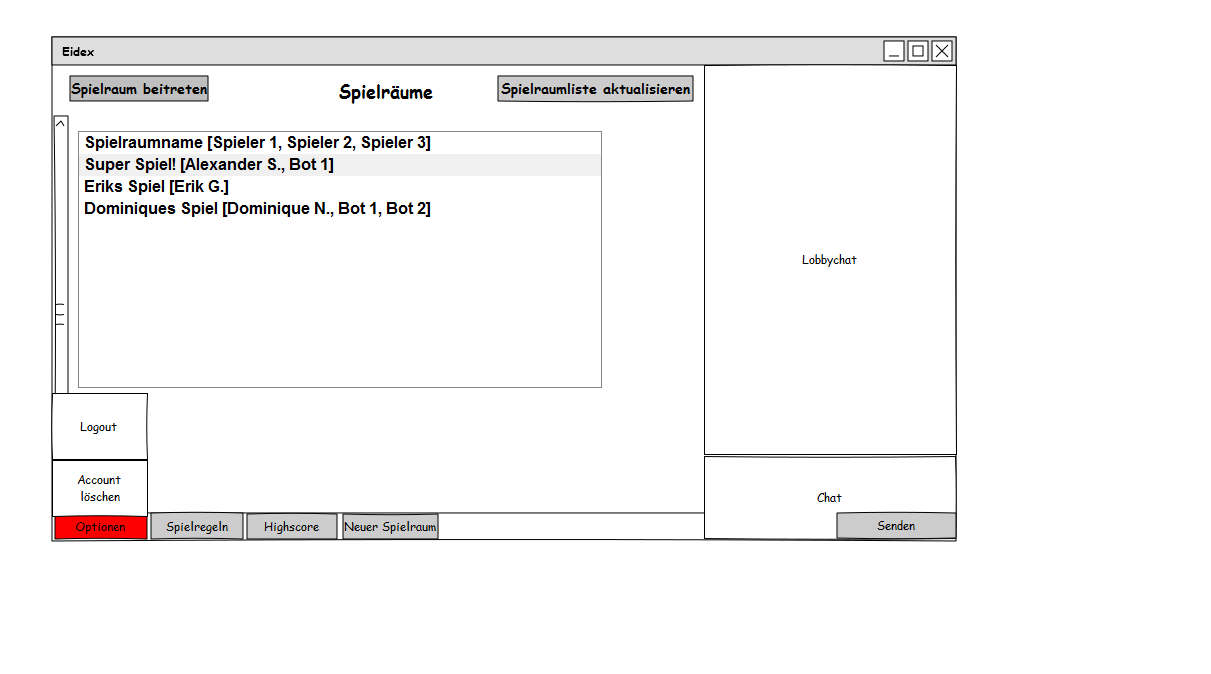
\includegraphics[width=170mm, height =140mm]{PencilProjectData/optionen}
		\caption{GUI Optionen}
	\end{figure}
	
	\begin{figure}
		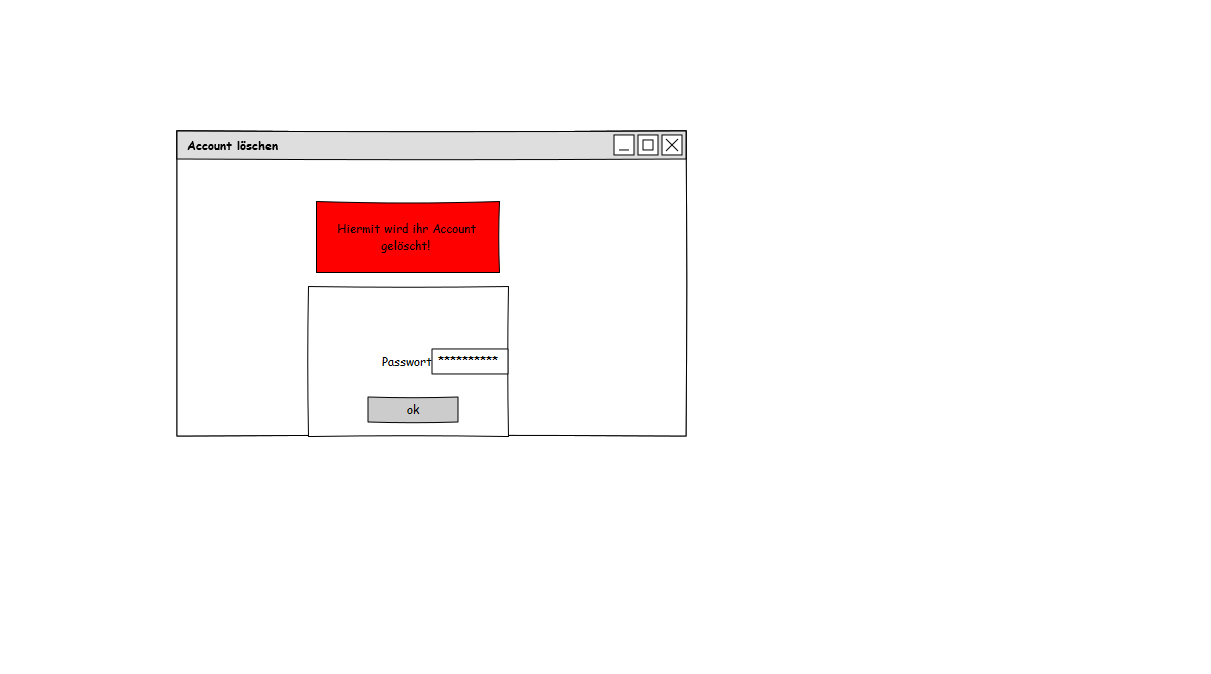
\includegraphics[width=170mm, height =140mm]{PencilProjectData/account_loeschen}
		\caption{GUI Account löschen}
	\end{figure}
	
	\begin{figure}
		\hspace*{-0.5cm}
		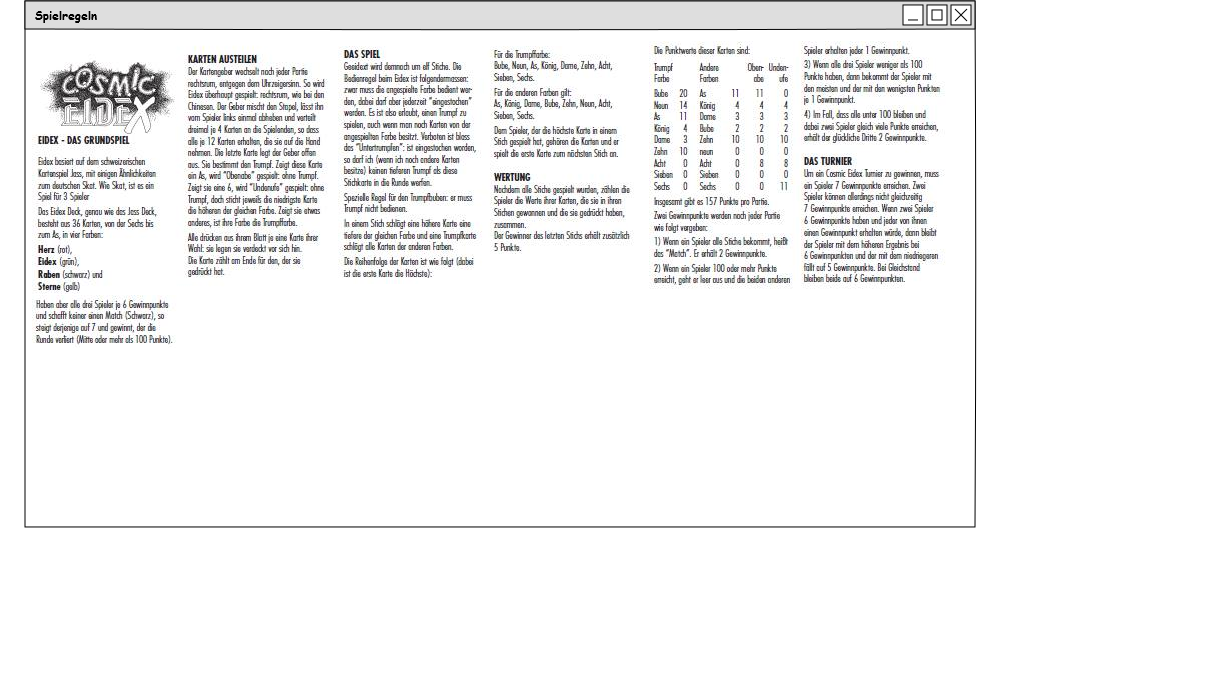
\includegraphics[width=170mm, height =140mm]{PencilProjectData/spielregeln}
		\caption{GUI Spielregeln}
	\end{figure}
	
	\begin{figure}
		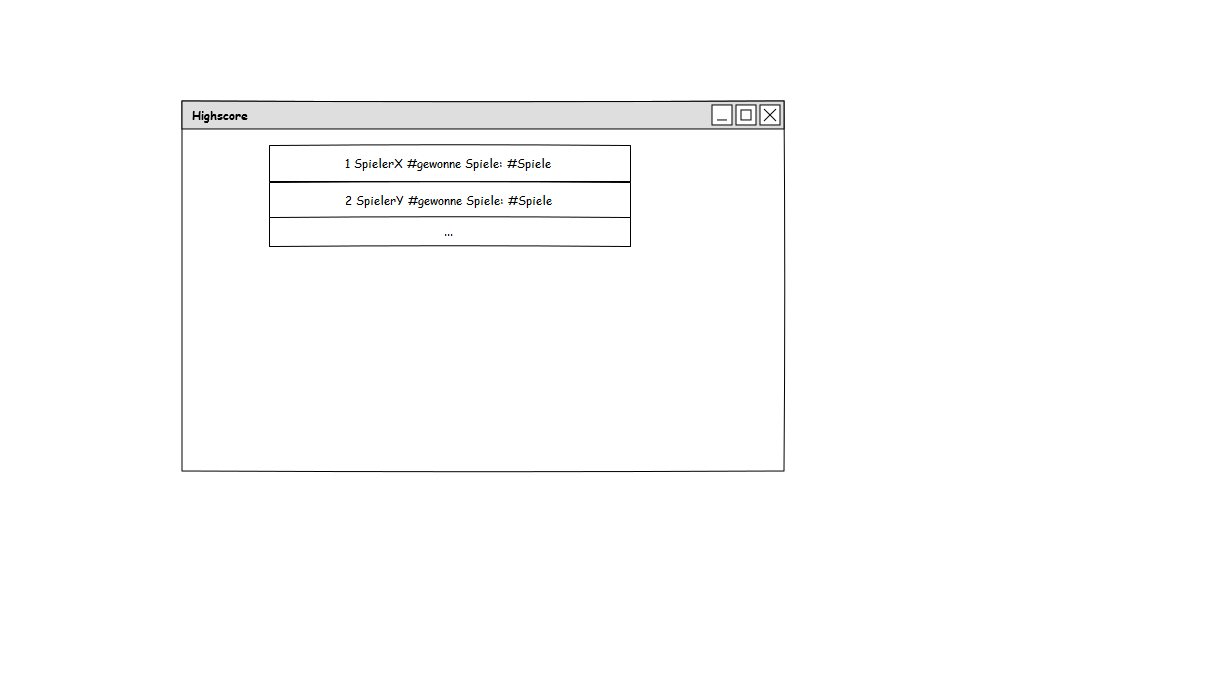
\includegraphics[width=170mm, height =140mm]{PencilProjectData/highscore}
		\caption{GUI Highscore}
	\end{figure}
	
	\begin{figure}
		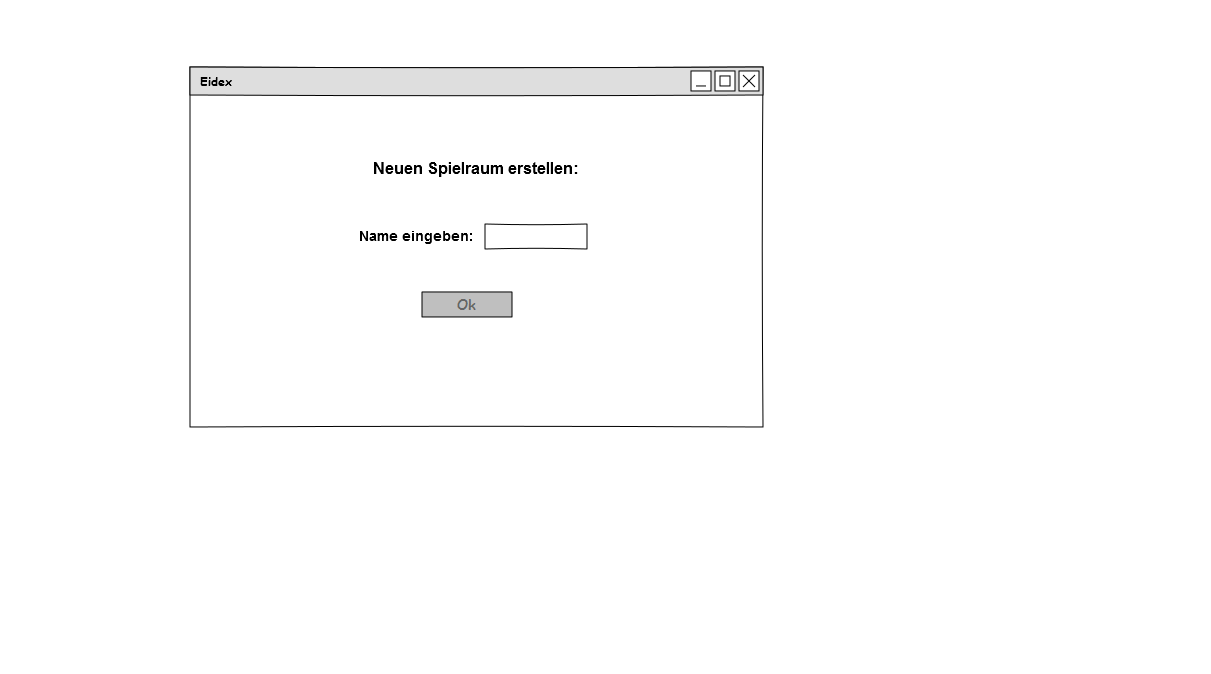
\includegraphics[width=170mm, height =140mm]{PencilProjectData/neuer_spielraum1}
		\caption{GUI neuer Spielraum}
	\end{figure}
	\begin{figure}
		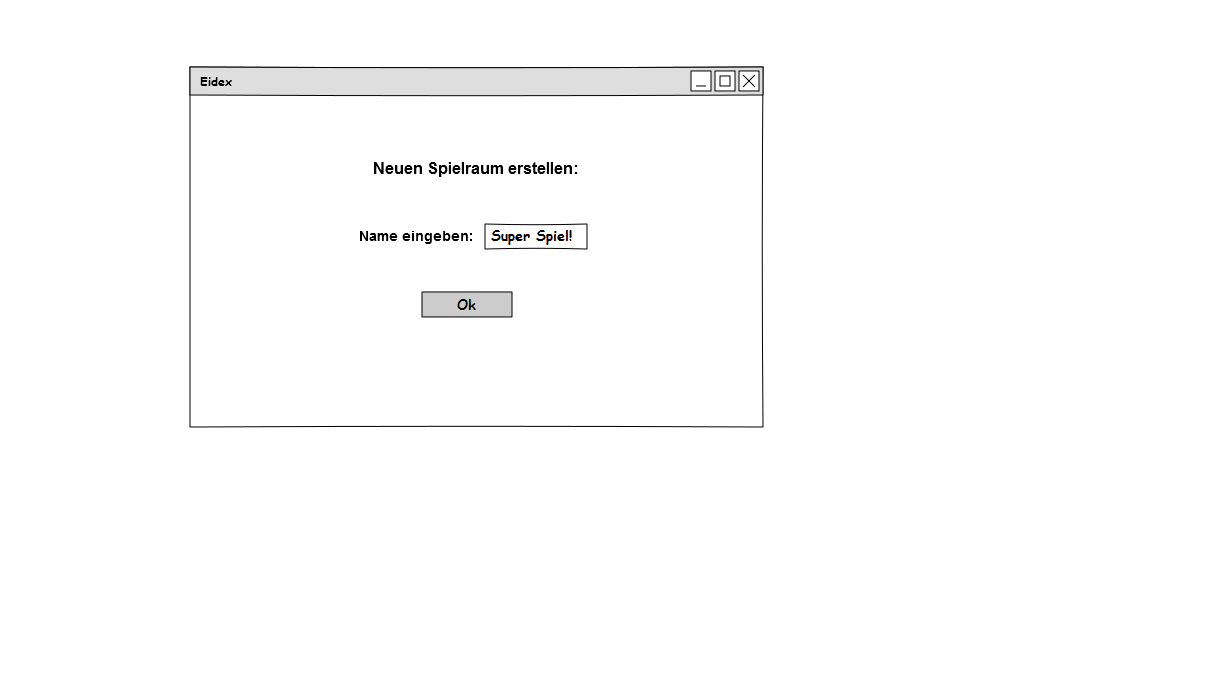
\includegraphics[width=170mm, height =140mm]{PencilProjectData/neuer_spielraum2}
		\caption{GUI neuer Spielraum}
	\end{figure}
	\begin{figure}
		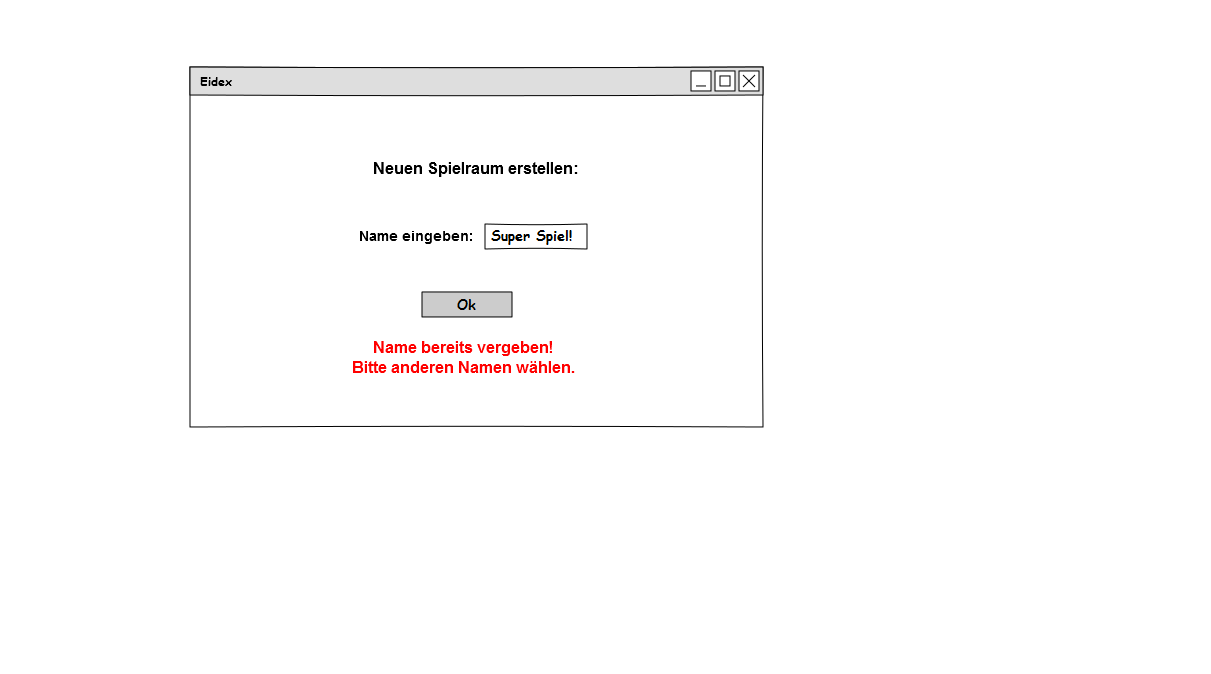
\includegraphics[width=170mm, height =140mm]{PencilProjectData/neuer_spielraum3}
		\caption{GUI neuer Spielraum}
	\end{figure}
	
	\begin{figure}
		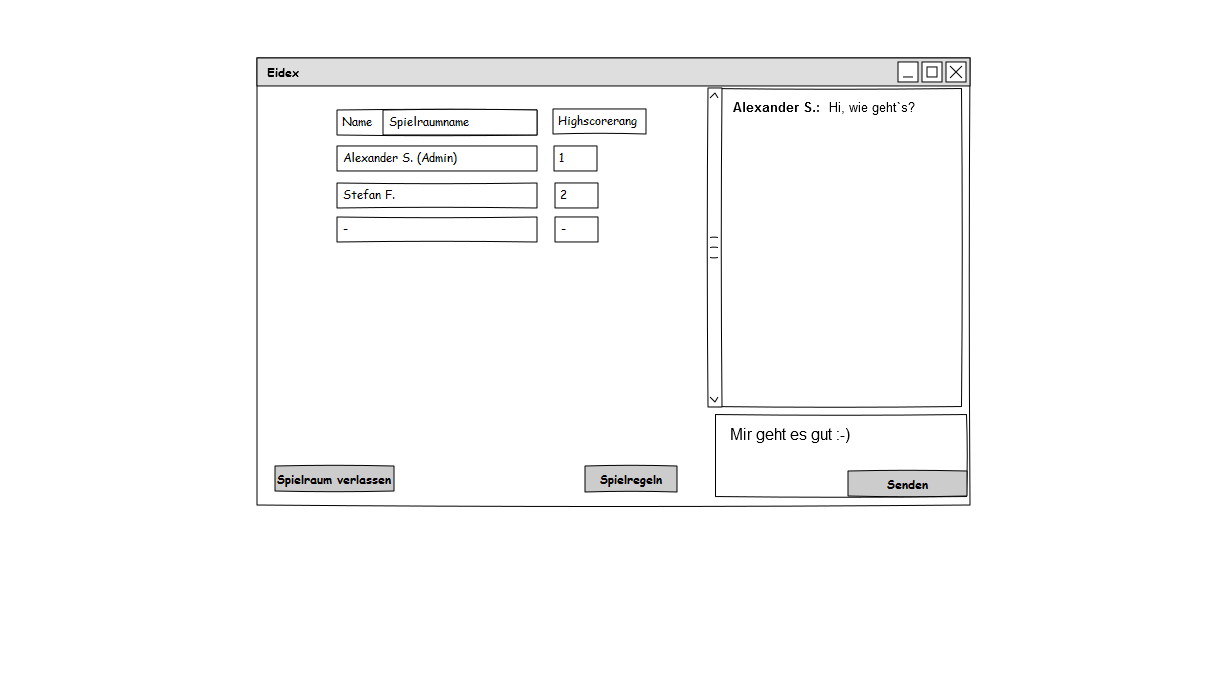
\includegraphics[width=170mm, height =140mm]{PencilProjectData/spielrauminfos1}
		\caption{GUI Spielrauminfos}
	\end{figure}
	
	\begin{figure}
		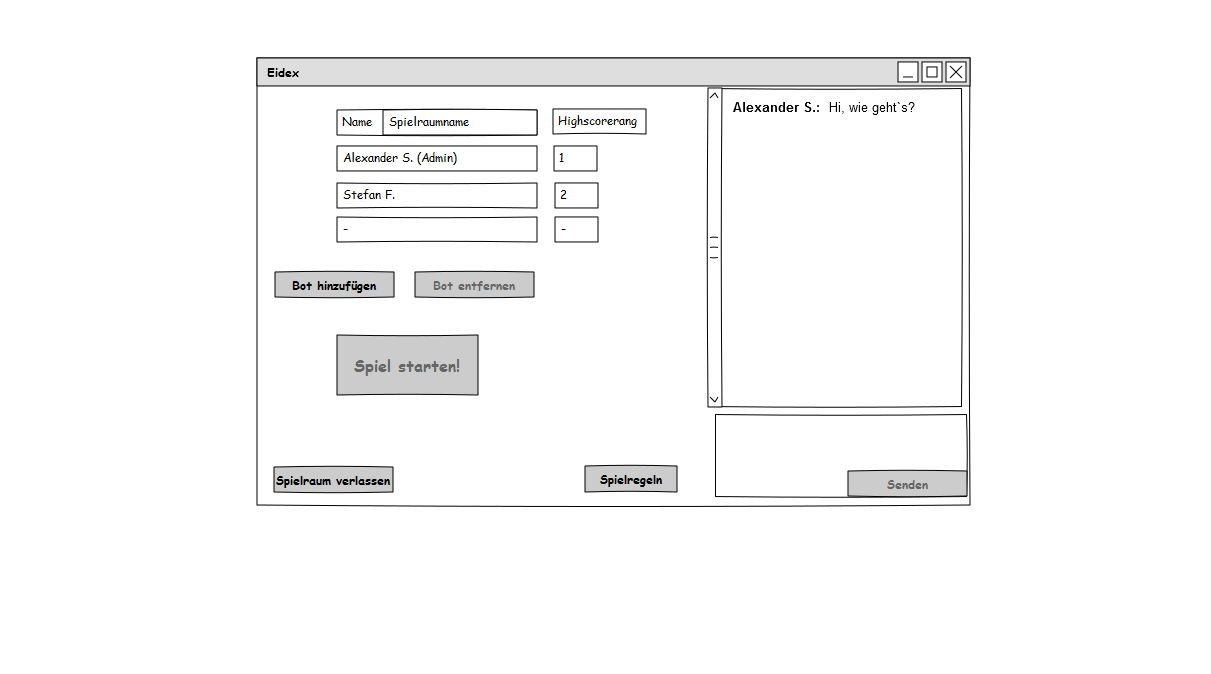
\includegraphics[width=170mm, height =140mm]{PencilProjectData/spielrauminfosAdmin1}
		\caption{GUI Spielrauminfos}
	\end{figure}

	\begin{figure}
		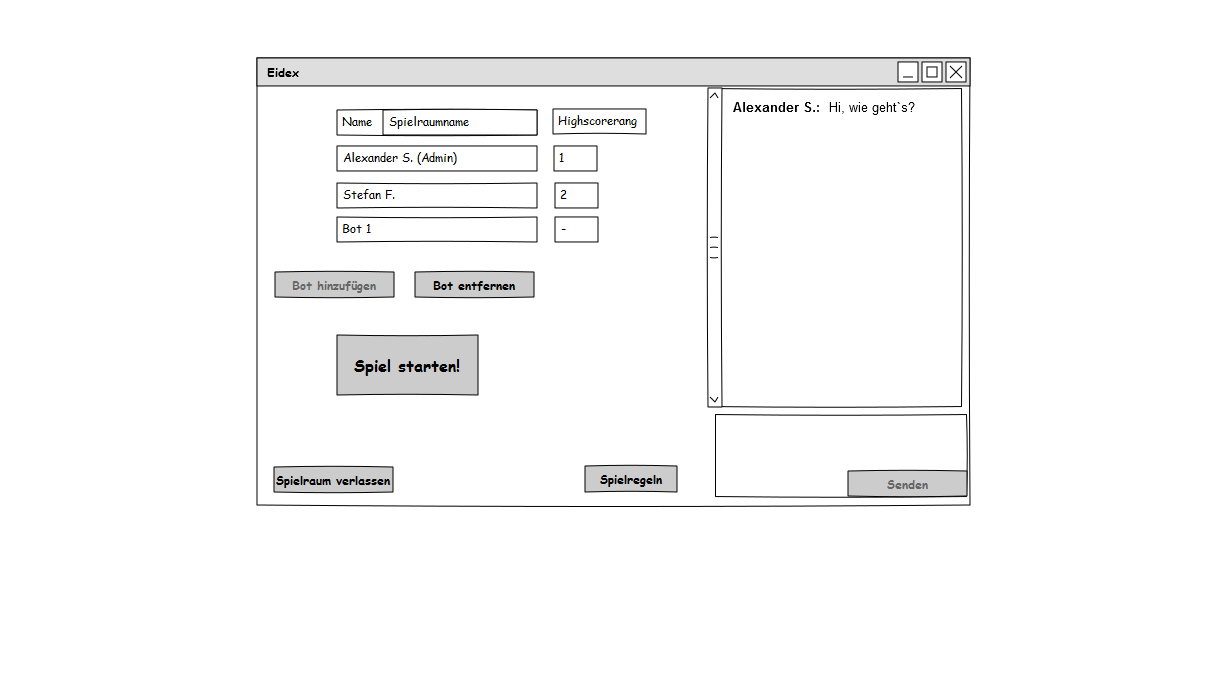
\includegraphics[width=170mm, height =140mm]{PencilProjectData/spielrauminfosAdmin2}
		\caption{GUI Spielrauminfos}
	\end{figure}
	
	\begin{figure}
		\hspace*{-1.5cm}
		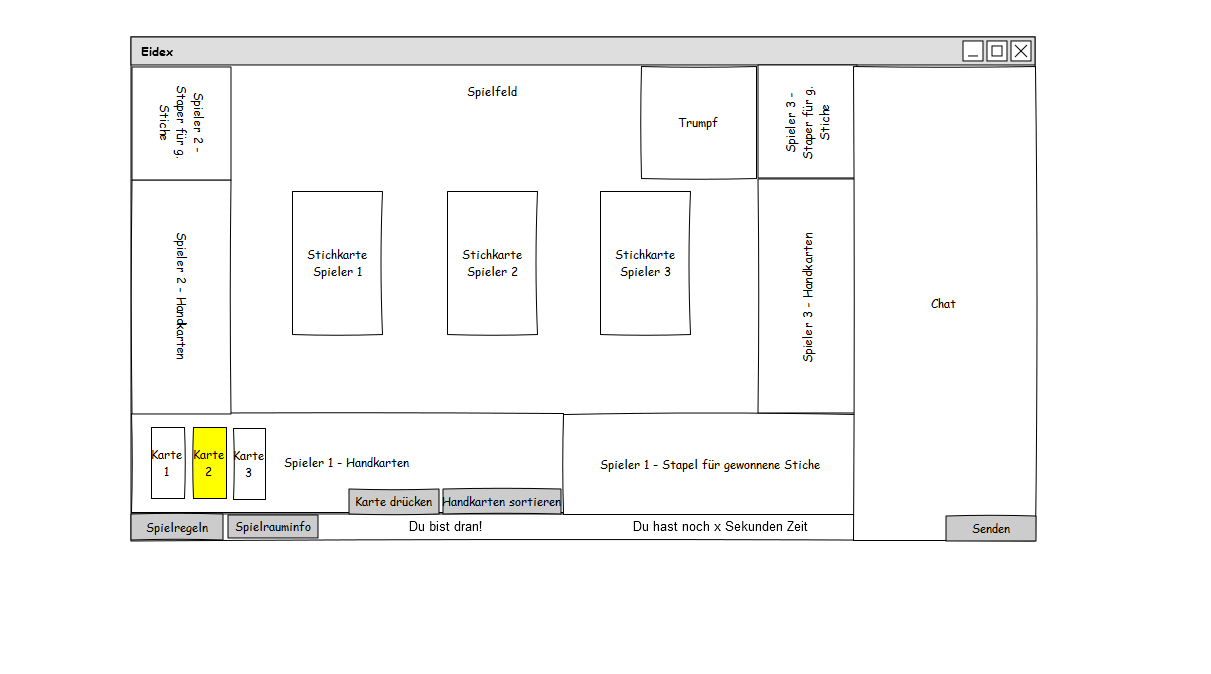
\includegraphics[width=170mm, height =140mm]{PencilProjectData/imSpiel_neu}
		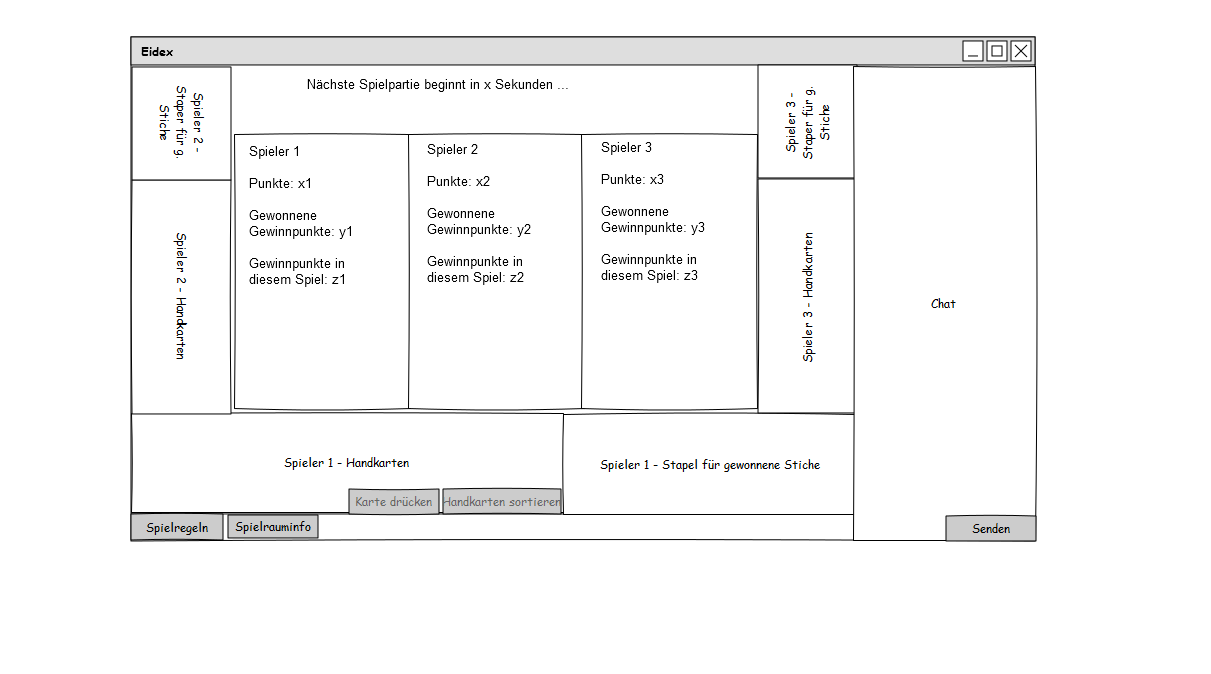
\includegraphics[width=170mm, height =140mm]{PencilProjectData/spielpartie_beendet}
		\caption{GUI Spielpartie beendet}
		\caption{GUI im Spiel}
	\end{figure}



\end{center}

	
	
	
	